\newpage
\section{Morfeas ISO Channel Linker}
The ``Morfeas ISO Channel Linker" is an utility made to create ISO channels and link them with sensors.
It's can be accessed by the Morfeas WEB front page from the button with the anchor (
\includegraphics[height=.125in]{../art/anchor.png}).
At figure \ref{fig:ISOChannel_linker} shown an example of the ``Morfeas ISO Channel Linker" utility.

\begin{figure}[h]
\centering
	\fbox{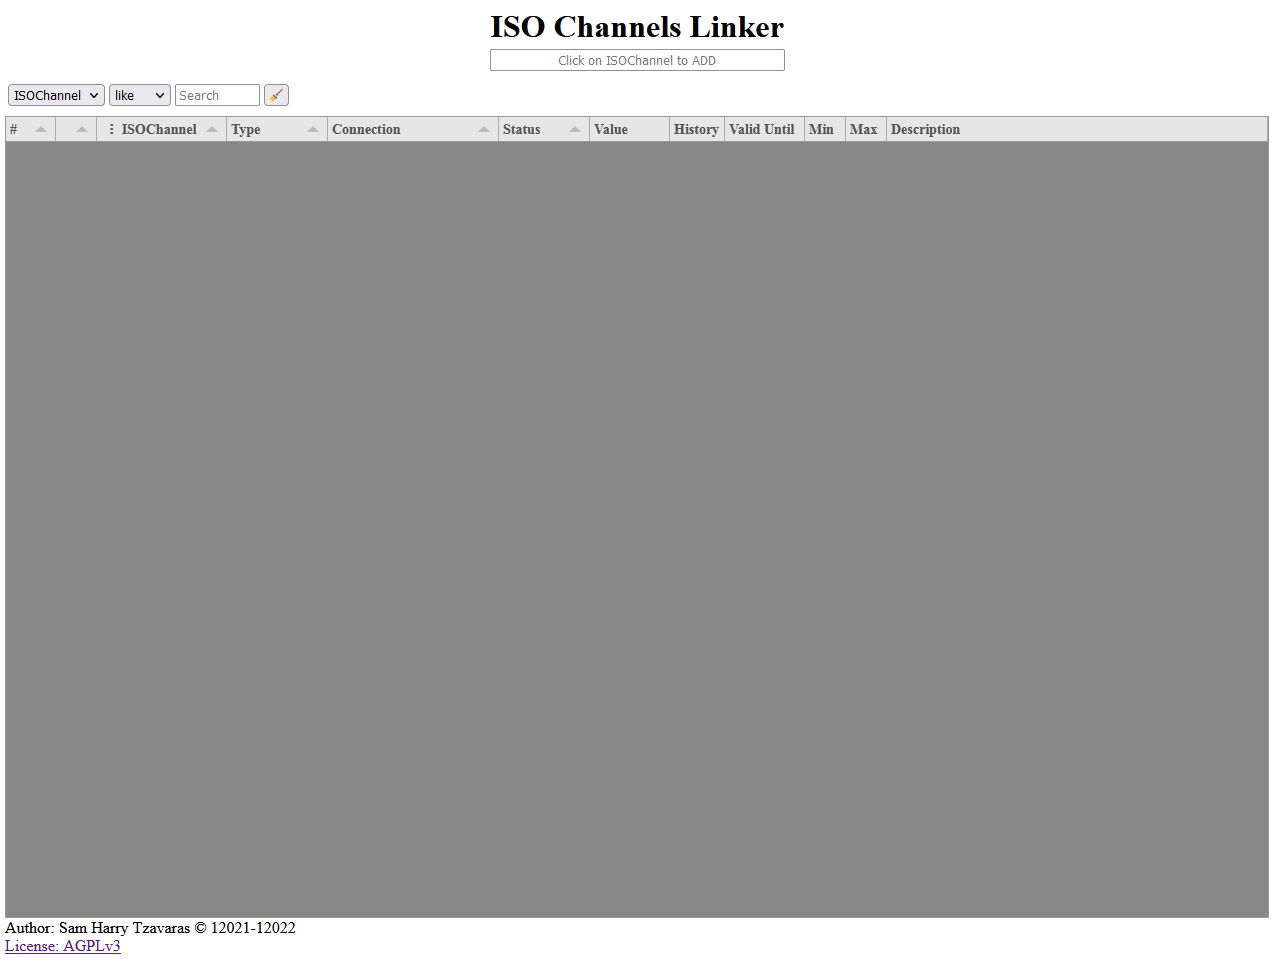
\includegraphics[width=3in,angle=0]{../art/Morfeas_web_if/Morfeas_WEB_ISOChannel_linker.png}}
	\caption{Morfeas ISO Channel Linker Utility}
	\label{fig:ISOChannel_linker}
\end{figure}
\noindent
The utility window split in three sections: the status bar, the filters section, and the ISO Channels table.\\

The status bar show the last update date if at least one channel exist,
or a message that informing the user to add channel(s).\\

The filter section, is filtering the ISO channels table, accordingly to the command from the user.
The filtering command is specified from the two drop-down lists and the text input field.
The first drop-down is selecting the column that the filtering will applied.
The second drop-down select the filter type; for most of the columns (except ``Min" and ``Max")
is ``like" and ``regex". The ``Like" filter type is filter and show all the elements in the specified column,
that contains the word in the search field, and similarly the ``regex" the fields that agree with the regular expression phrase.
For ``Min" and ``Max" the filter type change to a set of numerical comparing orders.
The button with the broom clean the filter.\\

The ISO Channels table is the configuration and presentation tool of the ``Morfeas ISO Channel Linker" utility.
It consist by 12 columns, with data for each ISO Channel.
The first column (from left) is show the order number of the ISO Channel.
The second column show with a color (table \ref{tab:col}) the status of each ISO Channel.
The third column contain the ISO Channel's name.
The forth and fifth contains the Connection type and path of the sensor that anchored to the ISO Channel.
Continue the sixth show the status of the anchored sensor, seventh the current value.
The eighth (History) contains a historical graph of past values of the sensors value, this graph show two minutes in past.
Next column show (if supported) the last valid date of the sensor.
The last three columns is the attributes of the ISO Channel; ``Min", ``Max" and ISO Channel's description.\\
Columns up to sixth can be shorted using the arrow at column name.
The shorting can be restored by clicking the filter clean button (broom).

\begin{table}[h!]
	\begin{center}
		\begin{tabular}{|c|l|}
			\hline
			\textbf{Color} & \textbf{Explanation}\\
			\hline
			Green & Okay\\
			\hline
			Orange & Calibration not valid\\
			\hline
			Red & Sensor warning\\
			\hline
			Black & OFF-Line/Disconnected\\
			\hline
		\end{tabular}
		\caption{Colors status}
		\label{tab:col}
	\end{center}
\end{table}

\subsection{Add a new ISO Channel}
To add a new ISO Channel the ISOChannels menu can be used (figure \ref{fig:ISOCH_menu}) or the shortcut \textbf{Ctrl}+\textbf{Alt}+\textbf{A}.

\begin{figure}[h]
\centering
	\fbox{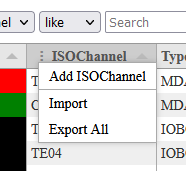
\includegraphics[width=2in,angle=0]{../art/Morfeas_web_if/Morfeas_WEB_ISOChannel_linker_menu.png}}
	\caption{ISOChannel's column menu}
	\label{fig:ISOCH_menu}
\end{figure}

By giving the ``Add ISOChannel" command (from menu or shortcut) a new window with the ``Link Creator" will appear (figure \ref{fig:ISOCH_new_link}).

\begin{figure}[h]
\centering
	\fbox{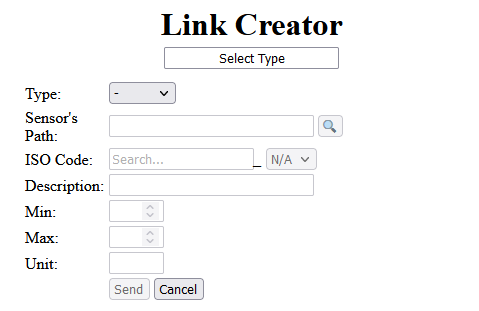
\includegraphics[width=3in,angle=0]{../art/Morfeas_web_if/Morfeas_WEB_ISOChannel_linker_link_creator.png}}
	\caption{ISO Channel Link Creator}
	\label{fig:ISOCH_new_link}
\end{figure}

The ``Link Creator" window request from the user to enter the information and attributes that related to the ISO Channel.
That's are: Type, Sensor's Path, ISO Code, Description, Min, Max and Unit.\\
The ``Type" entry is determinate the type of the sensor.
The ``Sensor's Path" is the logical path to the sensor, this determinated accordingly to the type of it.
For example for SDAQ type the path is constructed like ``CAN-f.Addr:XX.CH:XX".
In any case the ``Link Creator" will provide a hint related to the ``Type", or a message in case that no devices are available.
If the entry of ``Sensor's Path" is invalid will become red.
Also at the right of the ``Sensor's Path" entry is a button with a magnification glass on,
where if it clicked will open the ``Device Search" utility window (figure \ref{fig:Device_Search}).
The ``Device Search" utility provide a tree with the available sensors of the selected ``Type".
Any valid selection from the ``Device Search" utility will fill the ``Sensor's Path" entry.\\

The ``ISO Code" entry is specified the name of the ISO Channel.
The utility also hinting and autofill this and the following entries with values from the ``ISO Standard".
However, in manual entry the user is responsible to fill all the entries.\\

The ``Unit" entry is some of the values of the ``Type" entry will autofilled with the value that the sensor reporting.\\

If all the entries is validly filled the ``Send" button will become available, and on click will send and the ISOChannel.

\begin{figure}[h]
\centering
	\fbox{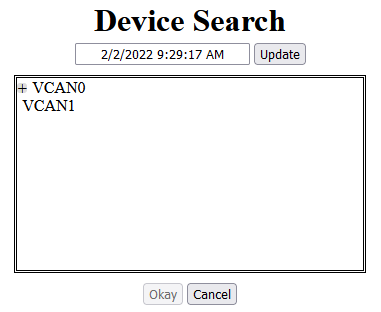
\includegraphics[width=2.5in,angle=0]{../art/Morfeas_web_if/Dev_search_win.png}}
	\caption{Device Search utility}
	\label{fig:Device_Search}
\end{figure}

\newpage
\subsection{Edit an ISO Channel}
The request of edit for an ISO Channel can be done by two ways.
Either by double click on the ISO Channel name,
or by right click (figure \ref{fig:right_click}) on the ISOChannel name and then click ``Edit".

\begin{figure}[h]
\centering
	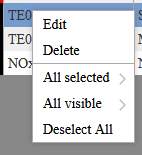
\includegraphics[width=1in,angle=0]{../art/Morfeas_web_if/right_click.png}
	\caption{ISO Channel Right Click menu}
	\label{fig:right_click}
\end{figure}

After the request of ISO Channel Edit, a new window (figure \ref{fig:edit_link}) with the ``Edit Link" utility will open.
The field that are available for edit are: Description, Min, Max, and Calibration date, calibration period, unit, if are specified from sensor type.
Also, if the ISO Channel that is under edit was in ``OFF-Line/Disconnected" state the Sensor's Path will be also available.

\begin{figure}[h]
\centering
	\fbox{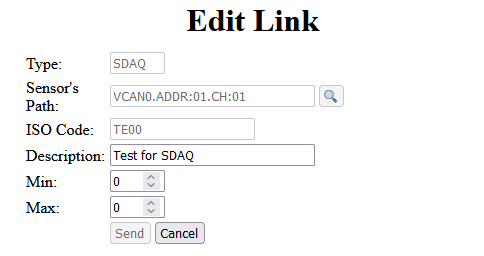
\includegraphics[width=3.5in,angle=0]{../art/Morfeas_web_if/Edit_link.png}}
	\caption{ISO Channel Edit Link Utility}
	\label{fig:edit_link}
\end{figure}

\newpage
\subsection{Delete ISO Channel(s)}
The deletion of one ore more ISO Channel from the table done in two ways, by selection and as group.
The by selection deletion done doing right click on the ISO Channel name that going to be deleted and select ``Delete".\\

The ``As group" deletion, done in two ways, by selected group and by visible group.
The selection of a group required first to make a selection group by clicking on the ISO Channel's row.
Then right click on any table's row, click on ``All selected" and then ``Delete".
Un-selection done by hitting ``\textbf{ESC}" key, or clicking on the filter clean button (broom).\\

The deletion of visible group have purpose to delete all the visible ISO Channel rows of the table.
Suppose that some filter have been applied before, then right click on some row, click "All visible" and then ``Delete".\\

In any case, before of a deletion request a verification message will appear.

\subsection{Export ISO Channels}
Exporting functionality of the Morfeas ISO Channel Linker Utility is the creation of an JSON file,
that contains the ISO Channels of the table or a selection. This file will save in the local computer by the browser.

To export all the ISO channels, use the menu of the ISO Channel column (figure \ref{fig:ISOCH_menu}),
 and Click ``Export All" or the shortcut \textbf{Ctrl}+\textbf{Alt}+\textbf{E}.
To export a selection of ISO channel it can use either a the ``All visible" (in combination with filtering),
or the ``All selected" (by have did a click selection) from the right click menu of the ISO Channel table (figure \ref{fig:right_click}).\\

For each case the exported file will be named accordingly to the selected operation together with the created date.

\subsection{Import ISO Channels}
The import of JSON file with ISOChannels can be done either from the ISOChannels column menu (figure \ref{fig:ISOCH_menu})
or by the shortcut \textbf{Ctrl}+\textbf{Alt}+\textbf{I}.
a new window with the import utility will be appeared (figure \ref{fig:imp_win}).
\begin{figure}[h]
\centering
	\fbox{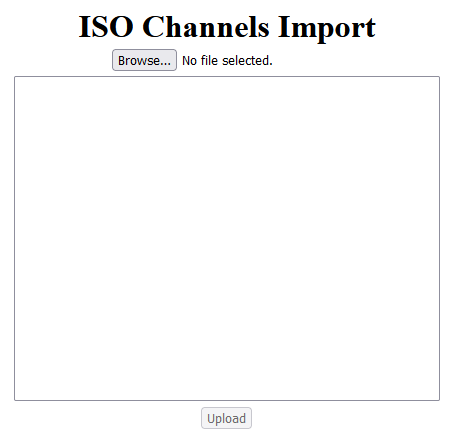
\includegraphics[width=2.5in,angle=0]{../art/Morfeas_web_if/import_win.png}}
	\caption{ISO Channel Import Utility}
	\label{fig:imp_win}
\end{figure}

From the import utility you select the file to be import by the ``Browse" button.
After the user's selection the validation procedure will start and the result of it will print in the logger.
In case that the validation pass with success the ``Upload" button will become available.
